
%(BEGIN_QUESTION)
% Copyright 2006, Tony R. Kuphaldt, released under the Creative Commons Attribution License (v 1.0)
% This means you may do almost anything with this work of mine, so long as you give me proper credit

Anta at en gassfyrt varmtvannsbereder styres manuelt, med en menneskelig operatør som observerer en temperaturindikator på varmtvannsutløpet og betjener en reguleringsventil for brenngass:
  
$$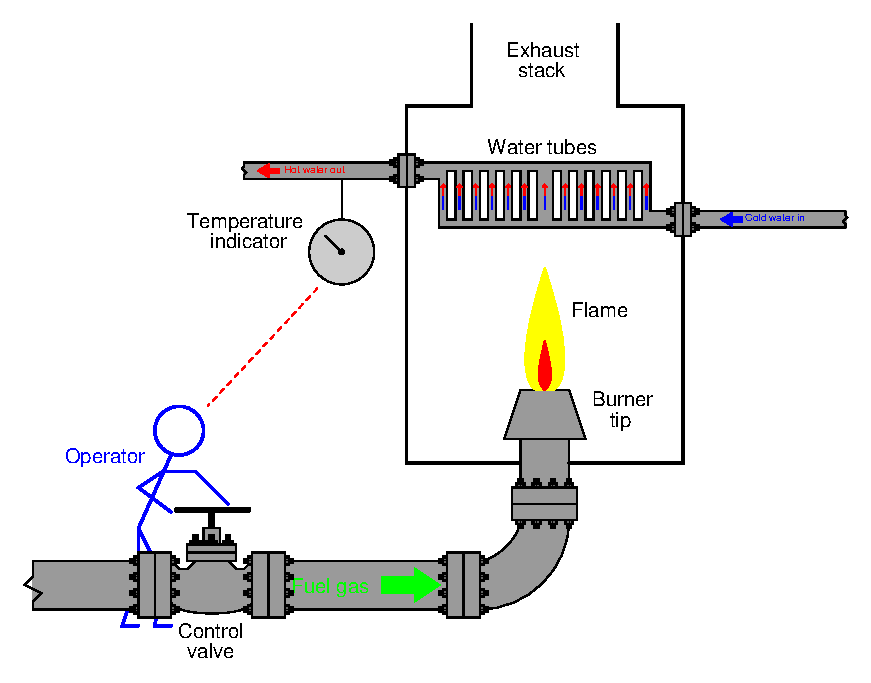
\includegraphics[width=15.5cm]{i01452x01.eps}$$

Spiller operatøren rollen som en {\it direktevirkende} regulator eller en {\it reversvirkende} regulator i dette prosessreguleringsscenarioet?

Identifiser også {\it prosessvariabelen}, {\it settpunktet} og {\it manipulert variabel} i dette manuelle reguleringssystemet.

\underbar{file i01452}
%(END_QUESTION)





%(BEGIN_ANSWER)

Den menneskelige operatøren spiller rollen som en {\it reversvirkende} regulator, fordi ventilbevegelsen må være motsatt av endringer i prosessvariabelen. Hvis vanntemperaturen for eksempel øker, bør operatøren bevege reguleringsventilen mer mot stengt.

\begin{itemize}
\item{} PV = vanntemperatur
\item{} SP = ønsket (mål-) vanntemperatur, i operatørens hode
\item{} MV = posisjonen til brenngassventilen
\end{itemize}

%(END_ANSWER)





%(BEGIN_NOTES)


%INDEX% Basics, control: direct versus reverse controller action

%(END_NOTES)

